\section{Setup}\label{section:setup}

In questa sezione vengono trattati i requisiti minimi necessari per l’utilizzo dell’applicazione ShopChain e successivamente come poter installare il prodotto in locale direttamente dal repository\glo
pubblico GitHub\glo del gruppo Yakuzaishi, accessibile al seguente link: \href{https://yakuzaishi-swe.github.io}{link al repository}.

\subsection{Requisiti di sistema}

Per far si che le operazioni di installazione e avvio del prodotto avvengano correttamente e che si possa
aver accesso a tutte le funzionalità, è necessario avere installati nella propria macchina i seguenti software.

\begin{table}[H]
	\centering
	\renewcommand{\arraystretch}{1.8}
	\rowcolors{2}{green!100!black!40}{green!100!black!30}
    \begin{tabular}{c | c | c}
		\rowcolor[HTML]{125E28}
		\multicolumn{1}{c}{\color[HTML]{FFFFFF} \textbf{Software}} &
        \multicolumn{1}{c}{\color[HTML]{FFFFFF} \textbf{Versione}} & 
		\multicolumn{1}{c}{\color[HTML]{FFFFFF} \textbf{Link al download}}   \\ \hline
        Docker & 4.9.0 & \href{https://www.docker.com/products/docker-desktop/}{https://www.docker.com/products/docker-desktop/} \\ \hline
    \end{tabular}
    \caption{Requisiti di sistema}
\end{table}

Grazie all'utilizzo di Docker\glo, abbiamo facilitato la procedura di setup dell'applicazione, in quanto Docker stesso si occupa di inizializzare tutte le tecnologie necessarie alla compilazione.

\subsection{Requisiti hardware}

Per avere delle prestazioni accettabili dell’applicazione è preferibile possedere almeno i seguenti componenti hardware.

\begin{table}[H]
	\centering
	\renewcommand{\arraystretch}{1.8}
	\rowcolors{2}{green!100!black!40}{green!100!black!30}
    \begin{tabular}{c | c}
		\rowcolor[HTML]{125E28}
		\multicolumn{1}{c}{\color[HTML]{FFFFFF} \textbf{Componente}} &
		\multicolumn{1}{c}{\color[HTML]{FFFFFF} \textbf{Requisito}}   \\ \hline
        RAM & 4GB DDR4 \\ \hline
        CPU & Processore 64-bit con Second Level Address Translation \href{https://en.wikipedia.org/wiki/Second_Level_Address_Translation}{(SLAT)} \\ \hline
        SSD (o HDD) & 3GB \\ \hline
    \end{tabular}
    \caption{Requisiti hardware}
\end{table}

\underline{\textbf{Attenzione!}} In alcune CPU la virtualizzazione utilizzata da Docker per avviarsi non è abilitata di default, per abilitarla si deve accedere al BIOS\glo\ di sistema, e attivare l'impostazione correlata.
Essendo gli ambienti BIOS molto variabili da macchina a macchina, non ci è possibile dare una indicazione precisa su dove trovare l'impostazione da cambiare, al seguente link troverete una guida generale di esempio: \href{https://www.bleepingcomputer.com/tutorials/how-to-enable-cpu-virtualization-in-your-computer-bios/}{CPU virtualization}.

È necessaria inoltre una connessione internet stabile per garantire un servizio ottimale, senza vincoli di banda.

\subsection{Browser}

L’applicazione è stata testata e quindi resa compatibile con le ultime versioni dei browser che supportano l'estensione Metamask\glo, il cui setup verrà discusso nella sezione §\ref{subsection:Metamask}.

\begin{table}[H]
	\centering
	\renewcommand{\arraystretch}{1.8}
	\rowcolors{2}{green!100!black!40}{green!100!black!30}
    \begin{tabular}{c | c}
    \rowcolor[HTML]{125E28}
	\multicolumn{1}{c}{\color[HTML]{FFFFFF} \textbf{Componente}} &
	\multicolumn{1}{c}{\color[HTML]{FFFFFF} \textbf{Requisito}}   \\ \hline
    Google Chrome & 98 \\ \hline
    Microsoft Edge & 98 \\ \hline
    Mozilla Firefox & 97 \\ \hline
    Brave Browser & 1.36 \\ \hline
    \end{tabular}
    \caption{Requisiti browser}
\end{table}

\subsection{Metamask} \label{subsection:Metamask}

L'applicazione fa uso del plugin Metamask\glo per la gestione dei wallet e dei pagamenti, 
al seguente link è possibile trovare la pagina ufficiale di download:
 \begin{center}
     \url{https://MetaMask.io/download/}
 \end{center}
 Alla pagina sarà presente un bottone con scritto \texttt{"Install MetaMask"}
 \begin{figure}[H]
    \centering
    \includegraphics[scale=0.3]{immagini/install-MetaMask.png}
    \caption{Pagina download MetaMask}
\end{figure}
\textbf{}\\
Cliccando il bottone si verrà reindirizzati alla seguente pagina web nella quale basterà cliccare il bottone \textit{"Aggiungi"}:
\begin{figure}[H]
    \centering
    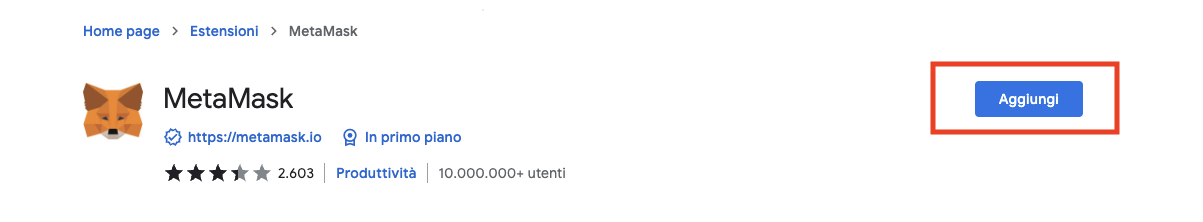
\includegraphics[scale=0.3]{immagini/MetaMaskExtensionPage.png}
    \caption{Aggiungere l'estensione MetaMask al browser (1)}
\end{figure}
\textbf{}\\
Si aprirà dunque il popup mostrato in seguito nel quale sarà sufficiente cliccare \texttt{"Aggiungi estensione"}
\begin{figure}[H]
    \centering
    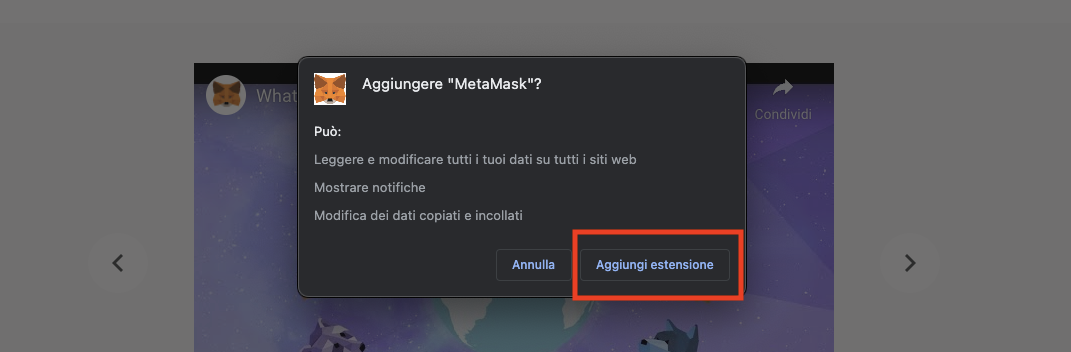
\includegraphics[scale=0.3]{immagini/AddExtenction.png}
    \caption{Aggiungere l'estensione MetaMask al browser (2)}
\end{figure}
\textbf{}\\
Una volta che l'estensione sarà stata aggiunta si verrà automaticamente reindirizzati alla pagina mostrata nella figura seguente nella quale sarà sufficiente cliccare \textit{Inizia}
\begin{figure}[H]
    \centering
    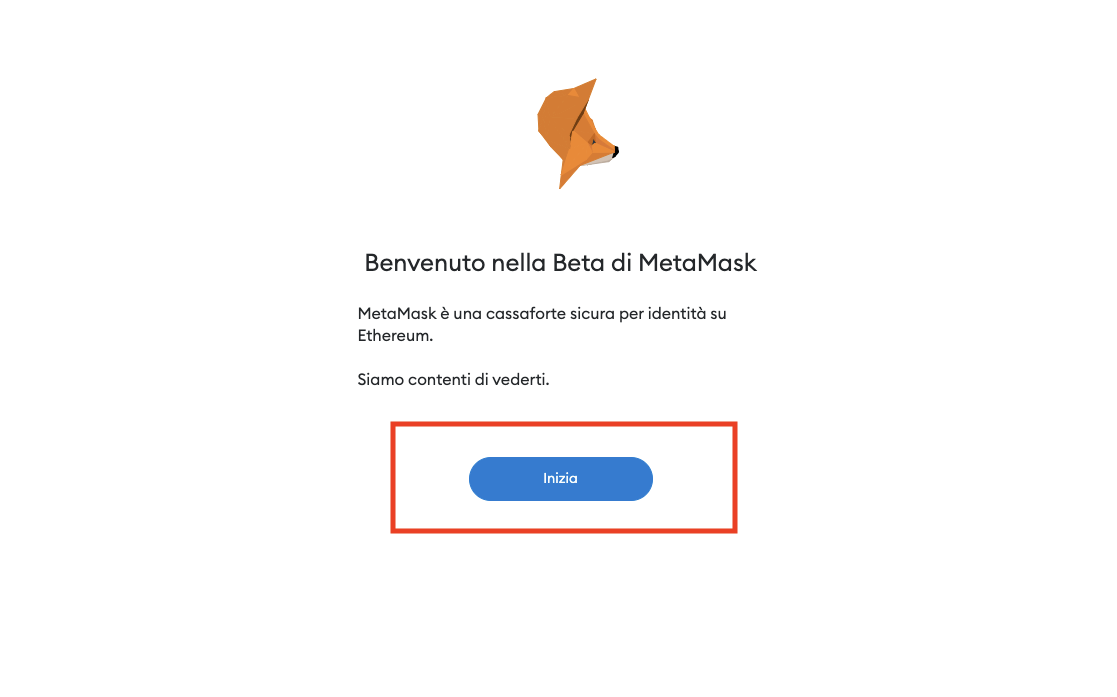
\includegraphics[scale=0.3]{immagini/startMetamask.png}
    \caption{Pagina iniziale MetaMask}
\end{figure}

\textbf{}\\
A questo punto non resta che scegliere se iniziare creando un nuovo portafoglio o se caricarne uno già esistente.

\begin{figure}[H]
    \centering
    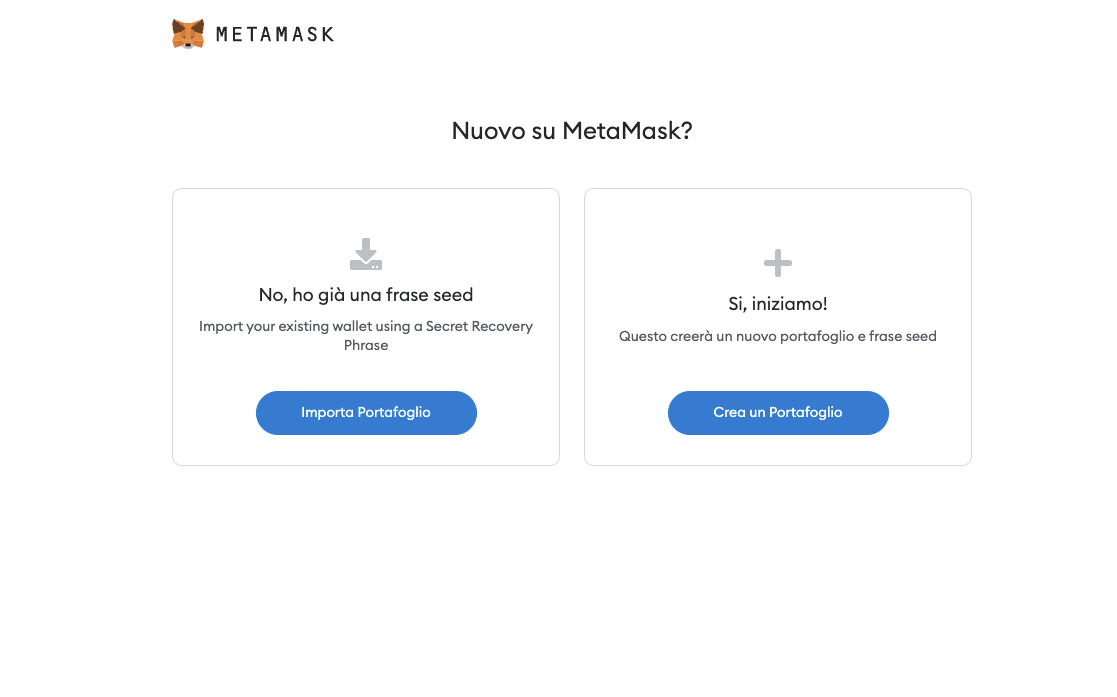
\includegraphics[scale=0.3]{immagini/chooseMetamask.png}
    \caption{Scelta iniziale MetaMask: crea/importa portafogli}
\end{figure}

\textbf{}\\
dopo aver scelto basterà seguire le semplici istruzioni riportate da MetaMask per completare il collegamento.

\subsubsection{Configurazione}
Per utilizzare l'applicazione \projectName{} è necessario disporre di un account MetaMask impostato sulla testnet Fantom.
Per aggiungere una nuova rete al proprio account MetaMask, cliccare sull'estensione MetaMask, quindi su \texttt{"Rete Ethereum Principale"}  e infine \texttt{"Aggiungi Rete"} come mostrato di seguito:
\begin{figure}[H]
    \centering
    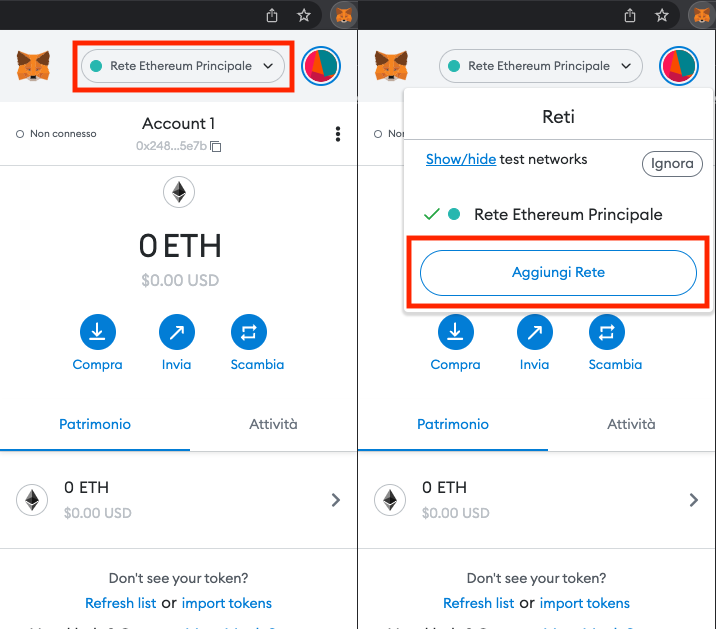
\includegraphics[scale=0.4]{immagini/Configuration.png}
    \caption{Inizio configurazione Fantom Testnet}
\end{figure}
\textbf{}\\
Si verrà reindirizzati a una pagina contenente un form da riempire come mostrato di seguito:
\begin{figure}[H]
    \centering
    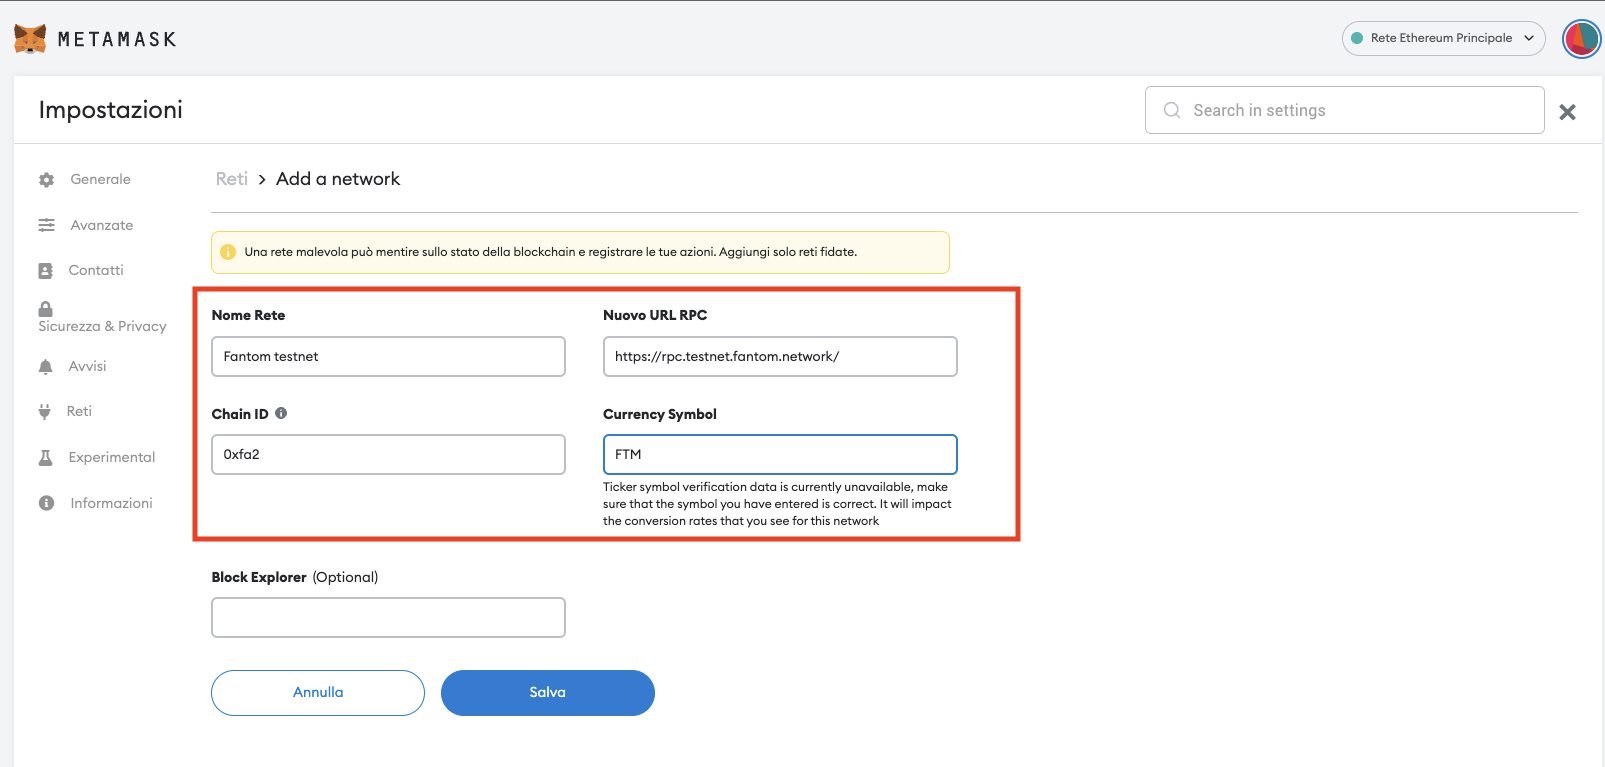
\includegraphics[scale=0.3]{immagini/ConfData.png}
    \caption{Form per l'aggiunta della rete Fantom Testnet}
\end{figure} 
\textbf{}\\
Per comodità vengono riportati i dati:
\begin{itemize}
    \item Network Name: Fantom testnet;
    \item New RPC Url: https://rpc.testnet.fantom.network/;
    \item ChainID: 0xfa2
    \item Symbol: FTM
\end{itemize}
Una volta riempito il form cliccare il tasto \texttt{Salva}.\\
A questo punto, una volta caricato denaro nel portafogli tramite la \href{https://faucet.fantom.network/}{Fantom faucet}, il setup sarà completo.\\\\
\underline{\textbf{Attenzione!}} Si raccomanda inoltre di notare che ciascuna operazione che prevede l'interazione con MetaMask (quali il pagamento, lo sblocco, il rimborso, la creazione della moneybox e il versamento di un contributo) prevedono il pagamento di gasfee, ovvero un ammontare variabile, generalmente piccolo, come commissione per il pagamento.\\
Tale ammontare è indipendente da \projectName{} o MetaMask, risulta invece essere indispensabile per permettere alla blockchain di registrare i blocchi all'interno dei quali è possibile reperire le transazioni.